%% This is an example first chapter.  You should put chapter/appendix that you
%% write into a separate file, and add a line \include{yourfilename} to
%% main.tex, where `yourfilename.tex' is the name of the chapter/appendix file.
%% You can process specific files by typing their names in at the 
%% \files=
%% prompt when you run the file main.tex through LaTeX.
\chapter{Deep Reinforcement Learning for Derivatives Pricing and Hedging}

\section{Motivations}
Previous work on derivatives pricing relies heavily on assumptions about the market and underlying stock movement to be consistent with theoretical standards for solving partial differential equations and deriving pricing models. For example, Monte Carlo simulations rely on the assumption that stock prices move according to a geometric Brownian motion stochastic process. As mentioned in Chapter 1, one of the most famous and widely-used options pricing models is the Black-Scholes Merton model. This framework is derived from a partial differential equation that also relies on many market condition assumptions that may not necessarily hold in real-world markets. For example, the model assumes through the option’s lifetime: no dividend payouts, constant risk-free interest rate, constant underlying volatility, and no transaction costs. The model also assumes the market has no-arbitrage conditions and there are no transaction costs.
\\ \\
However, these factors are all empirically dynamic and can affect underlying price movements and options premiums, but are not accounted for. These models serve as a good foundation for understanding some of the important factors that impact option prices, but in the real market, market dynamics can be affected by a large number of constantly changing factors. Many market frictions exist and are changing over time, which impact the value of financial derivatives. Furthermore, there are many types of different financial derivatives, each with unique properties, with options being one of the most popularly traded. A practical model would be developed on the basis of real market data that reflects the properties of market conditions on which the derivatives are traded, including transaction costs and other frictions.

\section{Derivatives Pricing Models}
To understand the fundamental ideas behind derivatives pricing and hedging, we first examine the theoretical approach with traditional options pricing models applied to risk-neutral pricing. As discussed in Chapter 1, the Black-Scholes model is the most widely-adopted foundation for understanding and analyzing option value and the factors that influence it. However, the model is not based on historical stocks and options data, but instead assumes the properties of stock price movement and makes many idealistic assumptions about market dynamics. Iterative improvements have been proposed to improve the framework, such as modeling using stochastic volatility as with the Heston model. Furthermore, derivatives pricing models have been developed for other types of assets other than equities, with different movement dynamics. 
\\ \\
For example, the Vasicek model is commonly used to model the evolution of interest rates to price interest rate derivatives. Another example is Black's model, an extension of the original Black-Scholes model, commonly used to price options on futures. Many models have been developed for various purposes and financial instruments, but they all rely on parametric assumptions instead of historical market data. This makes the basis of these models scientific, as the models are able to explain the specific factors that influence derivative prices, but potentially inaccurate as market dynamics are constantly changing. These models can also be applied in the context of devising hedging strategies to manage the risk of changes in the underlying factors.

\subsection{The Greeks}

Derivative prices are affected by a large number of variables that traders must constantly account for when developing trading and hedging strategies. There are some obvious factors that affect option prices that are captured, for example, by the Black-Scholes model: underlying price, time to expiration, volatility, and interest rate. The impact that a change in each of these aforementioned factors has on option prices is captured by the Greeks, which measure the sensitivity of option prices to these factors. Traditionally, traders and investors devised hedging strategies using the Greeks for the options they traded to account for the risk factors of option prices. Hence, various popular hedging methods used by many traders today include those such as delta hedging and gamma hedging, so that portfolios may remain delta or gamma neutral. The idea is to reduce the sensitivity of the options portfolio's value to underlying price movements as much as possible. A table of the most commonly-used Greeks and the corresponding definitions is displayed below.
\begin{table}[h]
\begin{center}
\begin{tabular}{c|c|c} 
\textbf{Greek} & \textbf{Value} & \textbf{Sensitivity to}\\[5pt]
$\Delta$ Delta & $\frac{\partial{V}}{\partial{S}}$ & Underlying Price\\[5pt]
$\Gamma$ Gamma & $\frac{\partial^2{V}}{\partial{S}^2}$ & Delta\\[5pt]
$\Theta$ Theta & $\frac{\partial{V}}{\partial{t}}$ & Time\\[5pt]
$\rho$ Rho & $\frac{\partial{V}}{\partial{r}}$ & Interest Rate\\[5pt]
$\nu$ Vega & $\frac{\partial{V}}{\partial{\sigma}}$ & Volatility\\[5pt]
\end{tabular}
\caption{The Option Greeks}
\end{center}
\end{table}

\noindent The option pricing models previously discussed provide a method to derive these Greeks for various options. Using the Greeks to devise hedging strategies is a reasonable approach in the absence of sufficient data and computational capacity \cite{deep-hedging-ppt}. However, this approach to solving the hedging problem is not as efficient as it could be, given the recent advancements in data-driven machine learning methods. Nonetheless, the Greek-based method is still widely practiced as its idea is intuitive, which is to adjust positions to reduce the impact of changes in the impactful factors.

\subsection{Dynamic Greek Hedging}

Perhaps one of the most practiced approaches used for hedging is delta-hedging, which involves adjusting the hedge ratio of a derivative position in response to changes in the underlying asset price, reducing the risk exposure of the position. The delta of an option represents its sensitivity to underlying price changes. Since underlying asset prices, stock prices, for example, are dynamically changing over time, it is important to dynamically rebalance portfolio positions to mitigate risks. Many traders look to maintain a delta-neutral position, in which the overall delta of the portfolio is zero, in order to mitigate risks in underlying price movements. However, due to transaction costs and other market frictions, perfect hedges are very difficult to achieve, and dynamically rebalancing delta positions can be extremely costly and often impractical.
\\ \\
Hedging is a problem that has many complexities to it based on various market risks. Delta hedging is widely known for its simplicity in interpretation and implementation. However, derivative prices are often impacted by a larger number of factors and market frictions that exist in real markets. Instead of the risk-neutral pricing framework, it may be beneficial to explore machine learning methods for solving the hedging problem to provide more accurate and robust results.

\section{Overview of Deep Reinforcement Learning}

\subsubsection{Reinforcement Learning}
Reinforcement learning (RL) is a method that overcomes many limitations of traditional machine learning. It involves exposing an agent to an environment with different states, available actions, the corresponding rewards for those actions, and letting the agent learn to maximize rewards through a Markov decision process. The power of reinforcement learning stems from its robustness and ability to quickly adapt to changing conditions relative to other types of machine learning methods. The results of state-of-the-art reinforcement learning methods have been promising, such as AlphaGo, the AI developed by DeepMind that beat the world Go champion, and ChatGPT, the language model developed by OpenAI that can answer questions and generate text in a human-like manner.
\\ \\
In an environment with current state $s_t$ at time $t$, an agent can perform a set of actions $a_t \in A$ that results in reward $r_t$ at time $t$ and moves the environment to the next state $s_{t+1}$. The environment is represented as a Markov decision process and the agent decides the optimal action to perform at each state $s_t$ according to its policy, $\pi: s_t \to a_t$. A diagram showing the reinforcement learning framework for the hedging problem is displayed below.
\\
\begin{figure}[h]
\centering
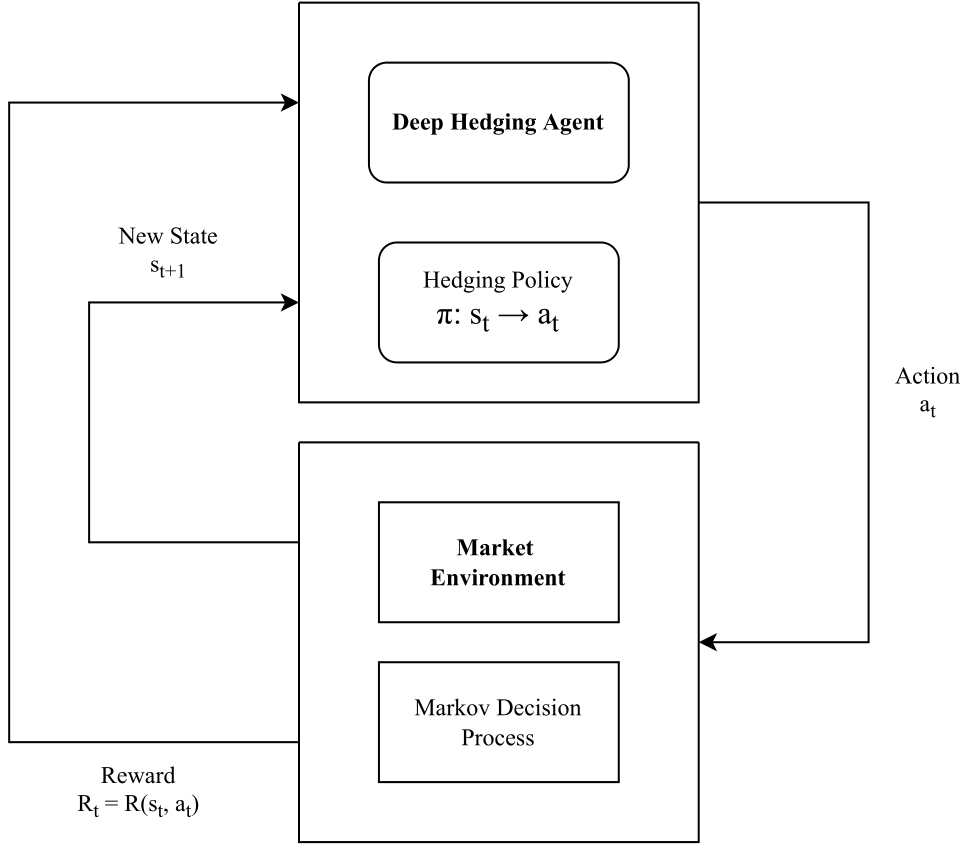
\includegraphics[width=11.5cm]{templates/assets/drl/rl.png}
\caption{Reinforcement Learning for Hedging Framework}
\end{figure}

\noindent This framework can be applied to a financial market environment with options trading with empirical economic and financial factors. The benefit of this approach is that it allows these factors to change dynamically across various time periods, which the agent will account for and gradually learn as it trains and explores the market environment. The goal is to implement a deep reinforcement learning system that can accurately price derivatives and dynamically hedge under actual market conditions and frictions. This can be done by using empirical data to learn the optimal policies for pricing and hedging through a policy gradient method. In the market environment, the agent will be given market conditions at each state and will incrementally learn the optimal hedging policy for correctly pricing derivatives and compute a PnL and Sharpe ratio for the dynamic hedging strategy as a reward function. Finding the optimal hedging policy, $\pi^\star$, results in maximizing the discounted cumulative reward:
\begin{equation}
    \pi^\star(s_t) = \max_{a_t \in A}{\mathbf{E}[\sum_{t=1}\gamma_tR_t|s_t, a_t]}
\end{equation}

\noindent with $\gamma_t$ as the discount factor at time $t$, as the agent will also want to account for the rewards from future states as the result of its actions. There are two ways to optimize the reinforcement learning agent. One way is to directly learn the expected rewards with a $Q$ function, $Q(s_t, a_t)=\mathbf{E}[\sum R_t|s_t, a_t]$ given a state and action pair $(s_t, a_t)$ and then using the $Q$ function to optimize the objective in equation 3.1. This method is commonly known as Q-learning, a form of value learning algorithm, to learn the value of an action at a particular state. The second method is to directly learn the optimal policy, $\pi^\star(s_t)$, without learning a mapping function of state and actions to rewards. This approach is known as policy learning and has produced promising results in state-of-the-art reinforcement learning algorithms.

\subsubsection{Combining Deep and Reinforcement Learning}
Early concepts of deep learning have been present since the 1940s, such as artificial neurons and perceptrons that could learn simple representations of data. However, because of early artificial neural networks' limited complexity combined with limitations in data and computing abilities, deep learning technology did not become widely adopted by institutions until the 21st century. In the present time with exponentially growing amounts of data and advanced processing units for fast computation and matrix algebra, the true potentials have deep learning have become gradually realized. The core of deep learning lies in its ability to learn incredibly complex and abstract relationships, both linear and non-linear, from vast amounts of data and be able to make accurate predictions using the learned representation. Often when the amount of data is enormous and highly dimensional, deep learning has proven to be significantly more effective compared to traditional forms of statistical learning.
\\ \\
Nevertheless, deep learning on its own has limitations, particularly in the context of modeling and predicting financial markets. Deep learning learns from the data it is provided but suffers from data drift, when the underlying distributions of the data change, and concept drift, when the actual factors that influence predictions changes. Because of these issues and the dynamic nature of the markets, it is difficult to develop a sustainable systematic framework for investing and hedging based solely on deep learning methods. However, combining the prediction power of deep learning with the robustness and flexibility of reinforcement learning, known as deep reinforcement learning, may yield much better results when applied to the financial markets. 
\\ \\
There are various state-of-the-art deep reinforcement learning algorithms that have recently been developed and have seen success in many applications, from playing games to autonomous driving. Deep Q-networks (DQN) is one type of algorithm that uses deep neural networks to approximate $Q$ values as previously described. This framework was first used by DeepMind \cite{dqn} to play Atari games by using a convolutional neural network to learn the value function of future rewards based on the game pixels. Another successful algorithm is known as proximal policy optimization (PPO) \cite{ppo}, a value function learning-based method, which has performed relatively similar or better than other state-of-the-art algorithms. Both of these deep reinforcement learning algorithms, and many others, can be applied to training agents to learn optimal hedging policies. Petter Kolm et al. demonstrate how proximal policy optimization can outperform traditional delta hedging and other deep reinforcement learning algorithms in finding the optimal hedging policy and optimizing PnL, training time, and amount of data required for training \cite{drl-ppo}.
\\
In a simplified world with only a limited number of states of the market, traditional reinforcement learning may be used, since the state-action-reward combinations are easily computed. However, in environments such as the financial markets, there are a very large number of states, with combinations of different factors including risk-free rates, stock movements, costs, etc. To account for the large dimensionality and complexity, this study examines the use of deep reinforcement learning methods to learn the states and rewards of the market by fitting a deep neural network on empirical data and using the learned states and rewards to train a reinforcement learning agent. The deep reinforcement learning framework for hedging is displayed below.
\begin{figure}[h]
\centering
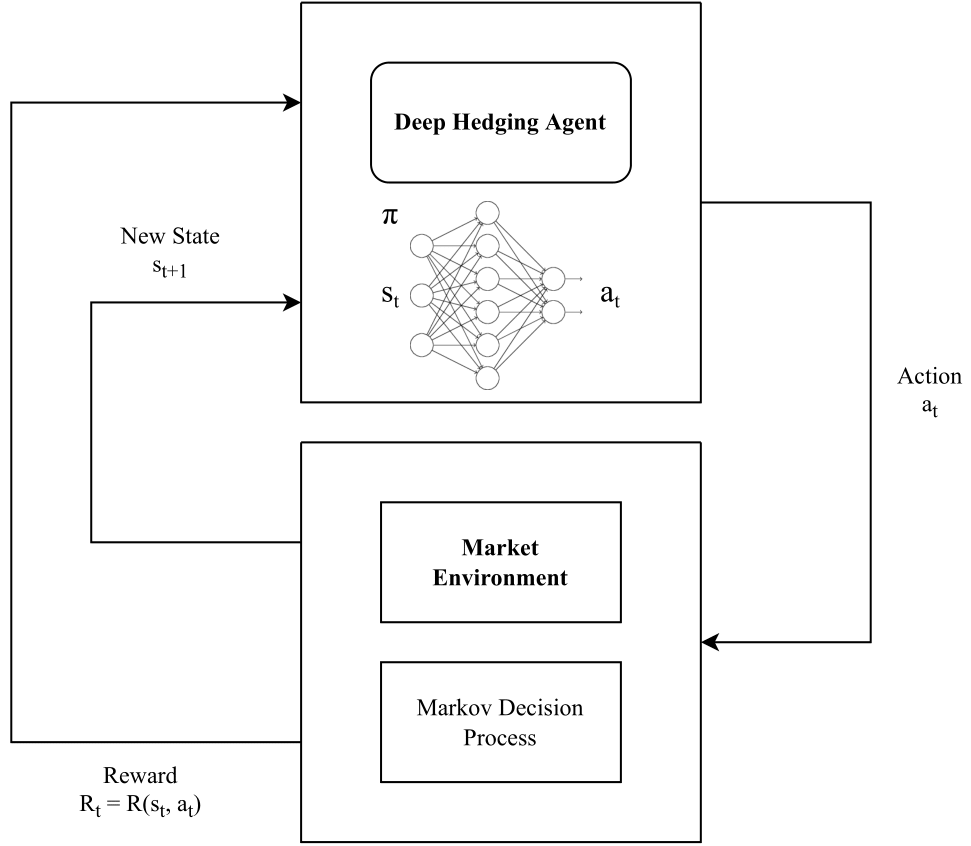
\includegraphics[width=11.5cm]{templates/assets/drl/drl.png}
\caption{Deep Reinforcement Learning for Hedging Framework}
\end{figure}

\subsection{Model-Based vs. Model-Free}
Some investors try to understand the overall market structure and make trading decisions based on their understanding, while other investors base trading decisions on their past experiences of successes and failures. In the reinforcement learning methodology, agents can also learn in these two types of ways. The former way, where the agent tries to learn a model of the environment to make predictions on the consequences and resulting reward of its current actions is known as model-based reinforcement learning. In this approach, the agent predicts rewards before any action is taken. This allows the agent to predict the future outcome of its actions based on the model of the environment it has learned. However, this makes the agent greedy and the agent may carry out any action despite immediate consequences. Furthermore, the learned model of the environment may be inaccurate when environment dynamics change, leading the agent to make poor decisions. Financial markets are one example of an environment that is often unpredictable and constantly changing, and a representation of the overall market in the present day may not be representative of the next. Consequently, model-based approaches may have weaknesses when applied to solving financial problems, just as investors may find it difficult to consistently predict the outcomes of their trading decisions before those trades are actually made.
\\ \\
To account for the dynamic nature of the financial markets, it may be more appropriate for agents to optimize their policies based on the rewards after actions have been taken, just as investors examine their PnL and Sharpe ratios after trades are executed. The latter way, where the agent learns to optimize its policy solely on its experience interacting with the environment during the training process is known as model-free reinforcement learning. In the context of hedging policies, the agent will learn by executing various strategies and observing the results of those strategies to optimize its policy. This allows the agent to be more robust to changing market conditions and learn directly from experience in the market.

\subsection{Multi-Agent Reinforcement Learning}
Oftentimes, simulations are carried out by more than one agent. For example, in financial markets and exchanges, there are many market participants including traders and investors that are simultaneously trading with each other. The orders that are made and executed between these market participants contribute to price movements. However, understanding and being able to simulate the interactions between these market participants may be beneficial for determining optimal trade executions and strategies. These market participants can be represented as multiple agents in the reinforcement learning framework. Instead of just a single agent in the environment, the market environment consists of multiple agents competing against each other to achieve the maximum reward. The multi-agent deep reinforcement learning framework for multiple trading agents is displayed below.
\begin{figure}[h]
\centering
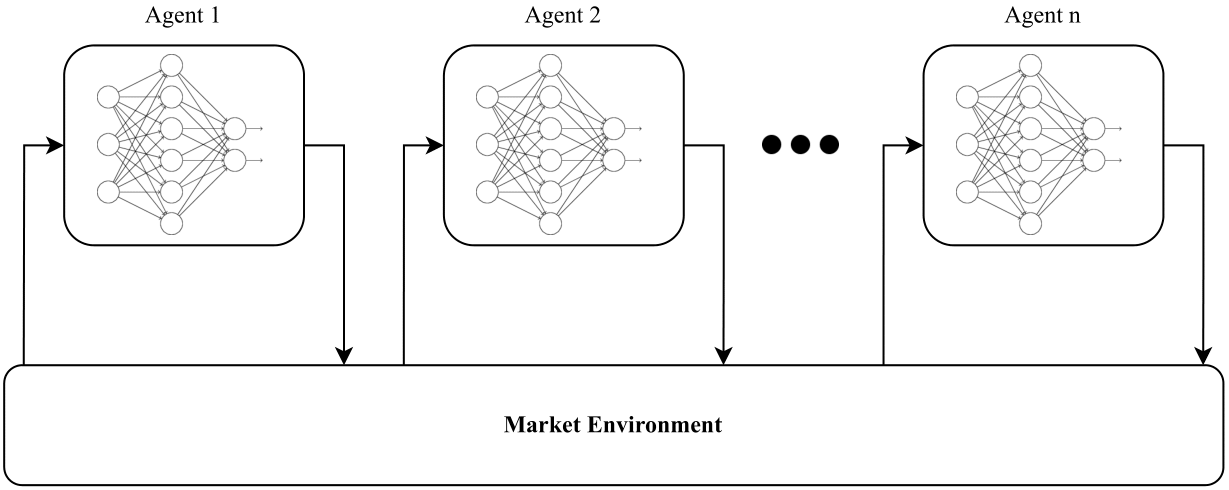
\includegraphics[width=12cm]{templates/assets/drl/madrl.png}
\caption{Multi-Agent Deep Reinforcement Learning Setup}
\end{figure}

\noindent Furthermore, it may be possible to represent all the agents in the system with a single generator agent that produces market transaction data. Victor Storchan et al. propose a framework called "MAS-GAN" \cite{mas-gan} to generate realistic market data by having a GAN represent the pool of market participants and learning to produce synthetic order book and bid-ask price data. This system can be used to not only train deep hedging algorithms on realistic multivariate time-series data but also evaluate their robustness to responses in the market, which is not accounted for in backtesting.

\section{Deep Hedging}

\subsection{The Hedging Problem}

Portfolios are constantly subject to a variety of risk factors that may significantly impact the portfolio's value and cause high volatility in returns. Hedging is a popular method to combat the risk that subjugates portfolios. The main idea behind this approach is to reduce risk and volatility by taking an offsetting position in another asset, such as a derivative of the underlying. However, hedging can be costly in a market with transaction costs and other frictions, along with the financial constraints of various investors. An effective hedging strategy must not only account for all the transaction costs involved but also all other imposed constraints.
\\ \\
Consider a discrete-time market at times $t_n \in T = \{0, t_1, t_2,..., t_N\}$ with a tradeable risk-free asset of price $B_n = e^{rt_n}$, and $D$ tradeable risky assets of prices $S_n = [S_n^1, S_n^2,..., S_n^D]$. There is a tradeable derivative in the market on the risky asset with a payoff equal to $\phi(S_n)$. In a complete market, it is possible to find a portfolio that fully replicates the payoff of a derivative. However, real markets are incomplete and strategies cannot replicate derivative payoffs, creating the objective of deciding the optimal policy for pricing and hedging traded derivatives to minimize the portfolio's value risk. Let the value of the portfolio at time $t_n$ be $V_{t_n}=B_{t_n}(V_{t_0}+DCG_{t_n})$ where $V_0$ is the initial capital and $DCG_n$ is the discounted cumulative gain of the hedging portfolio at time $t_n$. The asset allocations to each risky asset, $S_n$, is defined by $\vec\delta:=\{\delta_n\}^N_{n=0}$ resulting in the hedged portfolio. To find the optimal hedging policy that minimizes the hedged portfolio risk, the objective of the hedging problem then can be defined as:
\begin{equation}
    \delta^* = \min_{\delta \in \Delta}{\rho(V_{t_N}^\delta-\phi(S_{t_N}))}
\end{equation}
\noindent where $\delta^*$ is the optimal hedging policy that minimizes portfolio risk in a set of $\Delta$ possible hedging strategies. In this case, $\rho$ represents a risk measure such as value at risk, conditional value at risk, quadratic penalty, etc. The ultimate goal of the hedging problem is to optimize this objective and find the optimal hedging strategy under realistic market conditions including transaction costs and other frictions. However, because of the complexity and dimensionality of a realistic market environment, there is no closed-form solution for the optimal hedging strategy in equation 3.2. Instead, to approximate the optimal hedging policy $\delta^*$, the hedging strategies $\Delta$ can be parameterized as deep neural networks that can be trained to learn on data. 
\\
Ideally, to minimize a portfolio's risk exposure to underlying price movements, the portfolio should constantly be rebalanced to remain as close to delta-neutral as possible. However, as real markets typically have transaction costs, hedging can be very costly. Consequently, traditional Greek hedging methods such as delta hedging are not optimal and do not perform as well under real market conditions, having limited flexibility. Alternatively, a reinforcement learning approach can potentially learn the relationship between market states and the optimal hedging policy \cite{toronto-deep-hedging}.

\subsection{Applying Deep Reinforcement Learning to Hedging}
Deep hedging is a systematic framework for using deep reinforcement learning to learn the optimal policy for derivatives pricing and dynamic hedging based on the aggregation of market data. The deep hedging approach uses neural network representations to learn and optimize hedging policies. Hans Buehler et al. (2019) demonstrate in the original paper that neural networks can approximate well optimal hedging policies under general market conditions in the presence of frictions such as transaction costs. As some advantages of deep learning methods include being able to handle high dimensionality and being able to learn complex non-linear relationships, deep hedging has the potential to model these relationships between market factors and derivative prices. Deep hedging agents learn to dynamically adjust a portfolio's hedges in response to changing market conditions, which can make the algorithm significantly more robust and precise compared to traditional Greek hedging methods.
\\ \\
The goal of deep hedging is to minimize the overall risk of a portfolio by continuously adjusting the level of hedging in response to changes in market conditions. This involves the use of various hedging instruments including options and futures to hedge against potential large swings in the portfolio's value by trying to minimize the portfolio's risk. Deep hedging moves away from the risk-neutral world, where markets are complete and there is no arbitrage, to the real-world measure. As machine learning methods are data-driven, this framework can be applied to a wide range of financial assets, including stocks, bonds, commodities, currencies, and crypto.
\\
Reinforcement learning is an appropriate tool for the task of hedging because it can be adapted to work with different combinations of market conditions, portfolio complexities, and investment objectives. Unlike traditional optimization tasks, reinforcement learning agents remove the need to manually solve for optimal positions by interacting and learning the optimal strategy directly from a realistic market environment through trial and error. At a high level, deep hedging uses deep neural networks to predict the evolution of the markets and then uses this prediction to allow agents to learn how to dynamically adjust a portfolio's hedge positions to minimize risk.
\\ \\
Considering the hedging problem objective described in equation 3.2, a deep neural network can be used to represent hedging strategies and predict corresponding rewards in the market environment. This neural network can be used to allow the reinforcement learning agents to gradually learn the optimal hedging policy using this policy approximation framework. The structure of the hedging strategy neural network representation is displayed below.
\begin{figure}[h]
\centering
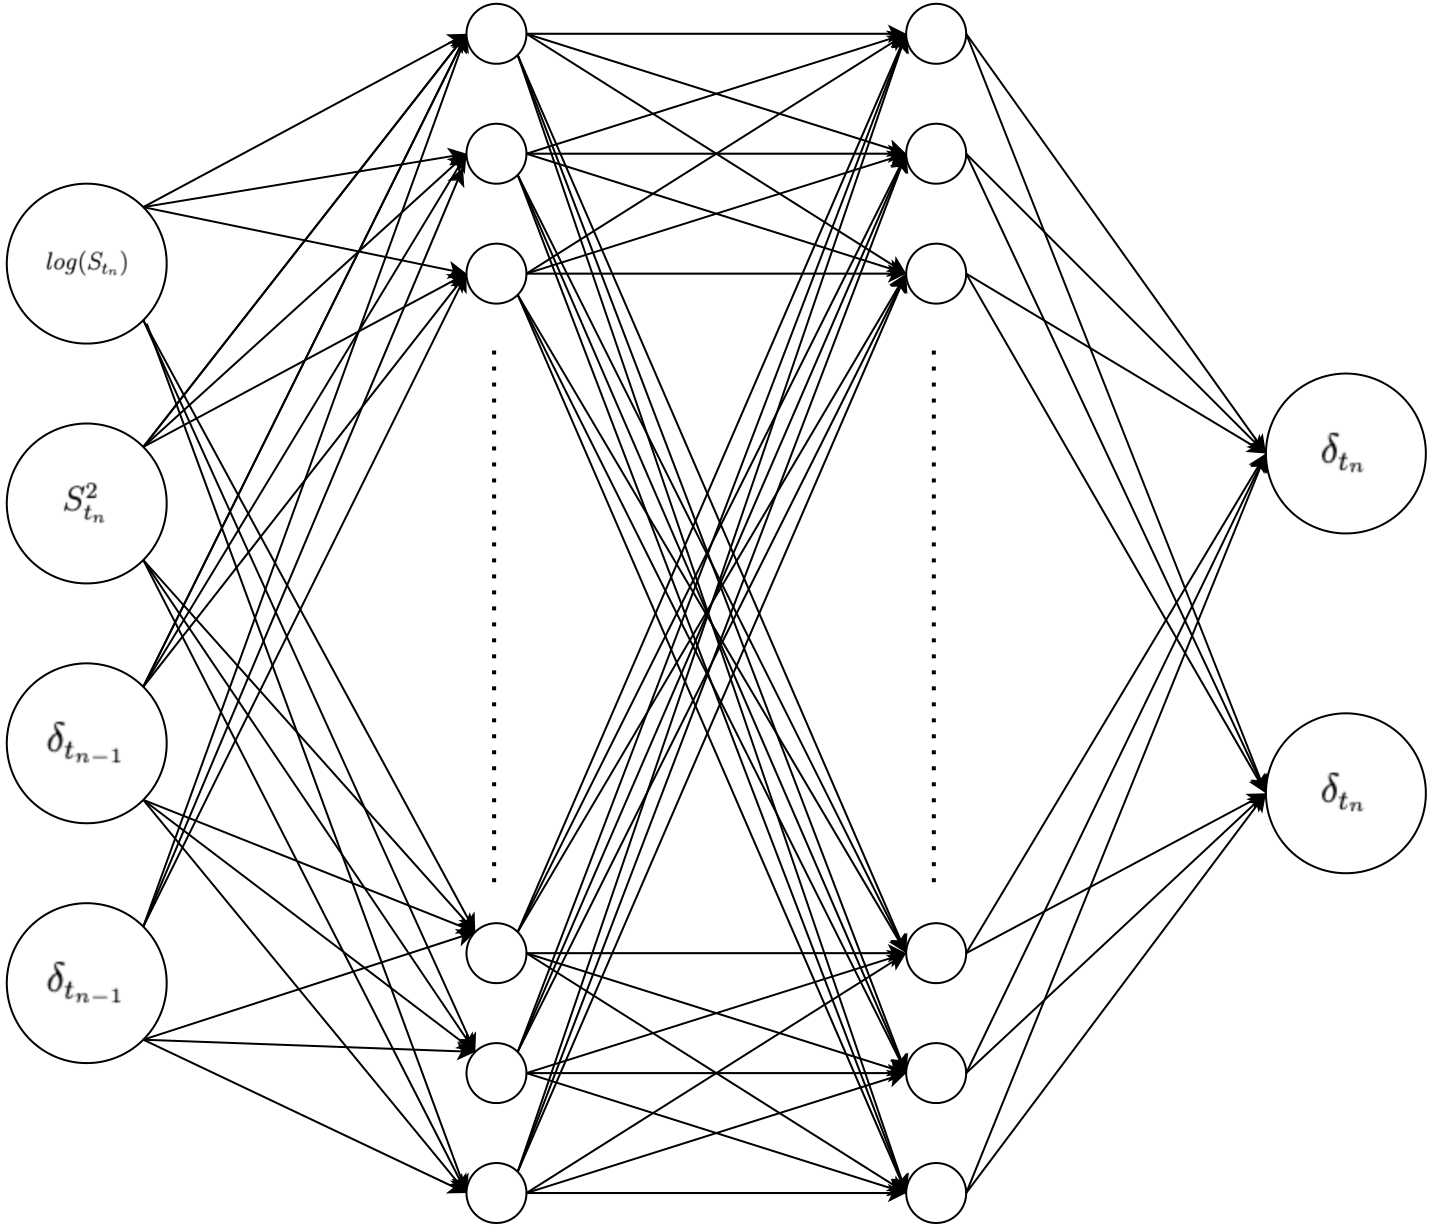
\includegraphics[width=10cm]{templates/assets/drl/dnn.png}
\caption{Learning Hedging Policy from Market State Deep Neural Network}
\end{figure}

\subsection{GAN-Based Market Environment}
The flexibility of the deep hedging framework allows the algorithm to learn from any type of market environment with any number of variables and factors. However, for the deep hedging algorithm to be practical for institutional investors and traders, the market environment must be as realistic and representative of real-world markets as possible. The original deep hedging system developed by Hans Buehler et al. (2019) was implemented under a Heston world with stochastic volatility, an improvement upon Black-Scholes, but is still parametric and makes assumptions about market dynamics. The authors suggest the use of a market simulator powered by machine learning methods, which may be more appropriate to represent real market conditions.
\\ \\
As explored in Chapter 2, GANs can be applied to the deep hedging framework by generating a diverse range of synthetic market scenarios that can be used to stress-test the hedging algorithms. The synthetic data that the GAN generates has statistical properties resembling real data. This data can help ensure that the hedging algorithm is robust and can handle a wide range of market conditions. GANs can be used to augment the training data for the hedging algorithm by generating additional synthetic data points that are representative of the real-world market. This can potentially help to improve the hedging algorithm's performance by increasing the amount and diversity of realistic training data available.
\\ \\
Market environments have frequently been simulated using a model such as Black-Scholes for the sake of simplicity and interoperability of market dynamics. In this implementation of deep hedging, the market environment is created by using GAN-based market simulation to capture the general properties of real markets, moving the system into the real-world measure. This creates a non-parametric model of the market, removing the need for making various assumptions about market dynamics. The overall framework of multi-agent deep reinforcement learning and GAN-based market simulation for derivatives pricing and dynamic hedging is displayed below.
\begin{figure}[h]
\centering
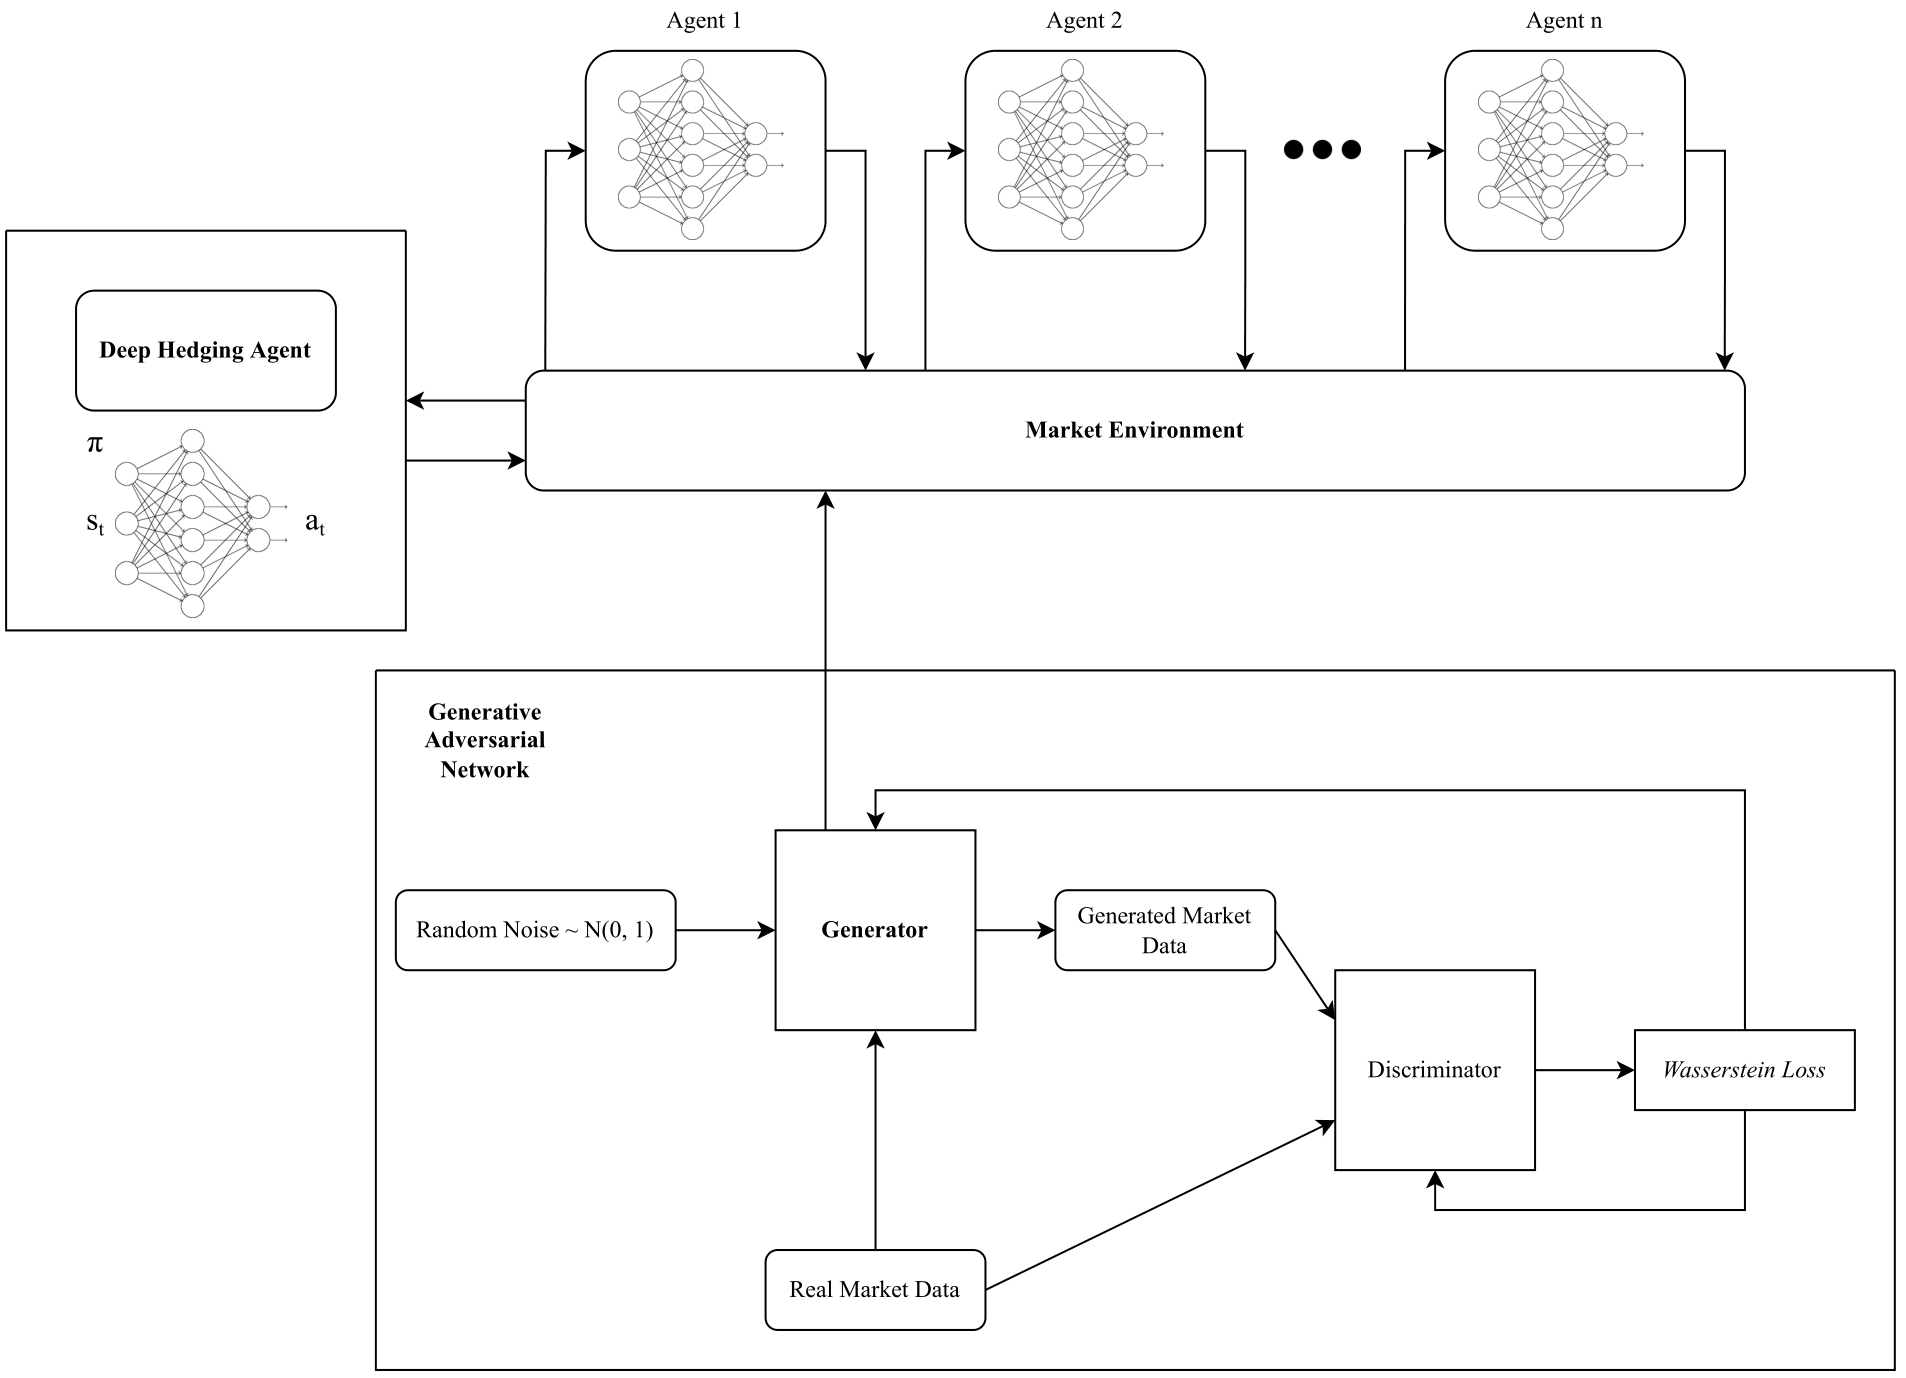
\includegraphics[width=14cm]{templates/assets/drl/rl_gan_combined.png}
\caption{Framework of Multi-Agent Deep Reinforcement Learning and GAN-Based Market Simulation for Derivatives Pricing and Dynamic Hedging}
\end{figure}

\section{Evaluating Deep Hedging Algorithms}
Using machine learning methods for derivatives pricing and hedging moves away from the risk-neutral pricing framework and does not require the assumptions and computations of a risk-neutral world. As previously mentioned, the reinforcement learning framework of deep hedging provides flexibility as to the type of market environment and constraints in the hedging problem. Previous works on using deep hedging methods have focused on the implementation of a Black-Scholes or Heston world. It is demonstrated by Hans Bühler et al. \cite{deep-hedging} that deep hedging is able to converge to the results of Black-Scholes delta in the absence of market frictions and transaction costs. However, using Black-Scholes or Heston to simulate underlying price movements still makes the deep hedging system model-based, as it relies on foundational assumptions about market dynamics. Instead, it may be more appropriate to use the GAN-based market simulator to represent the market environment.

\subsection{Black-Scholes World vs. GAN-Based Simulations}
The primary goal of using machine learning methods in deep hedging is to move away from the model-based and risk-neutral world framework that requires many assumptions about market dynamics. Ideally, a model-free system would learn and make decisions primarily on data instead of a model of the market, which is the purpose of the reinforcement learning system. To realize the true potential of machine learning and deep hedging methods for practical use in real-world markets, a model-free environment must be implemented, such as the one previously explored in Chapter 2, that does not require assumptions about how the market works. To observe the differences in using a Black-Scholes world and a GAN-based market simulator to train the deep hedging system, the realized hedged PnLs of the optimal hedging strategies can be visualized for both types of market environments. Running 100,000 market simulations with 30 time steps using both approaches yields the distribution of hedged PnLs displayed in the histogram below.
\begin{figure}[h]
\centering
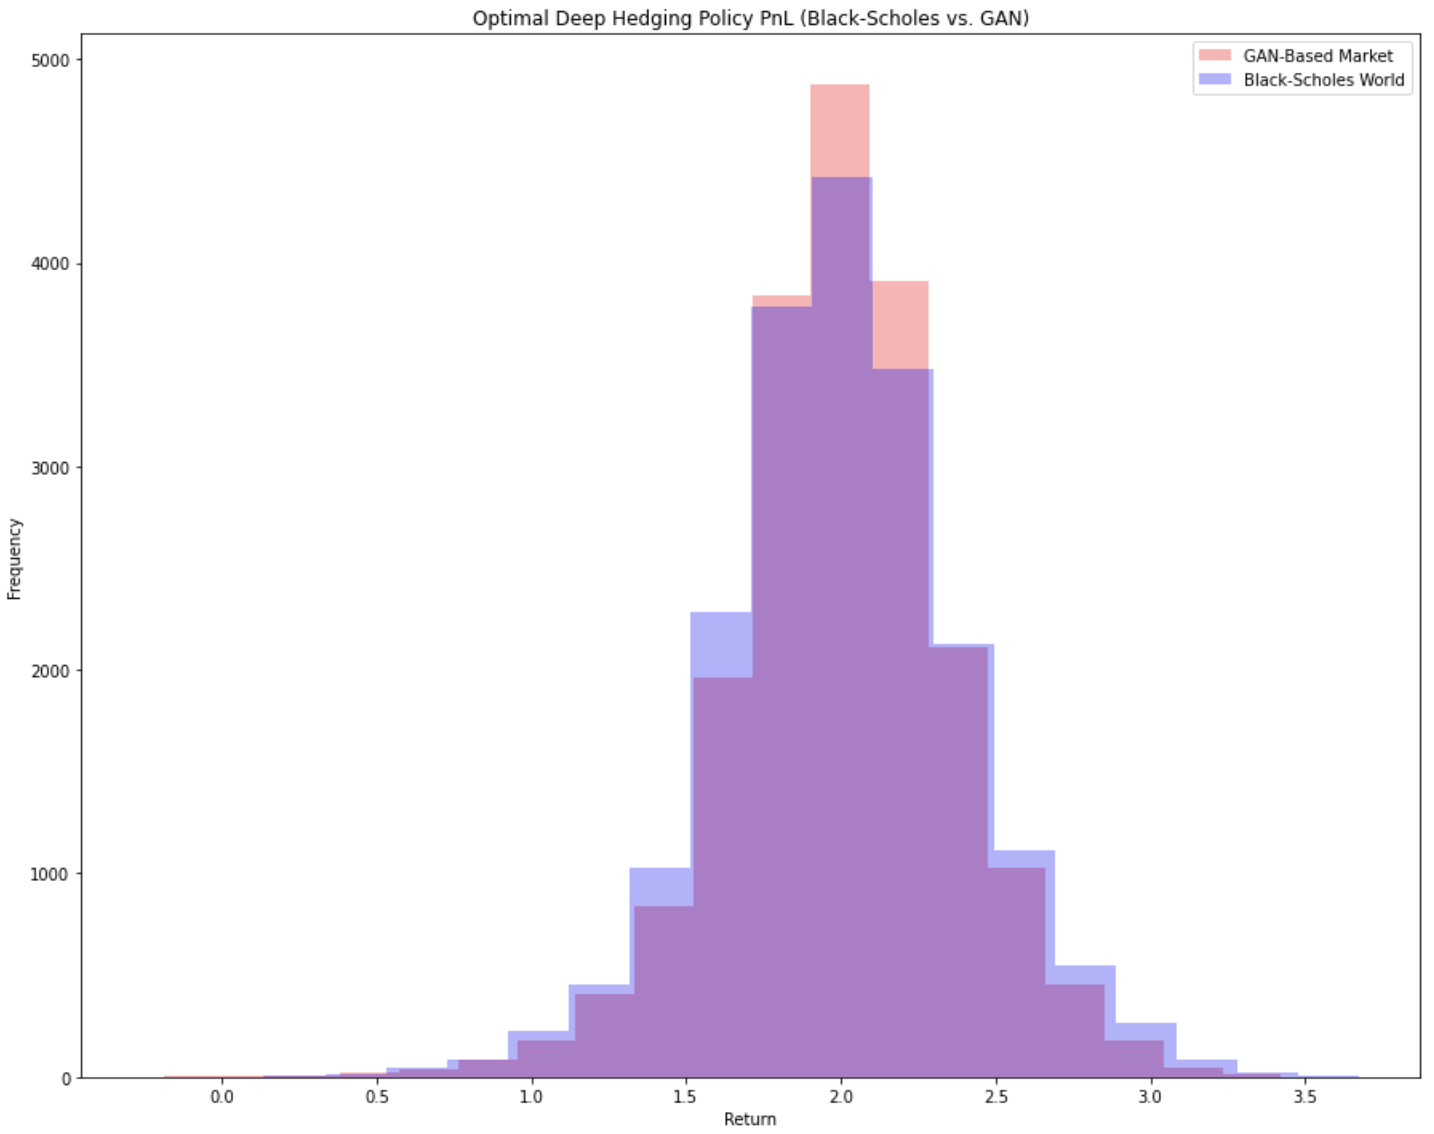
\includegraphics[width=13.5cm]{templates/assets/drl/hedge_pnl.png}
\caption{Optimal Deep Hedging Policy PnL (Black-Scholes vs. GAN)}
\end{figure}

\noindent Derivative prices are sensitive to changes in the underlying asset prices. This sensitivity, as described in Section 3.2.1, is referred to as the derivative's delta. The delta, or sensitivity to underlying price movements, of the hedged option can be visualized as a function of the underlying price over time. One of the goals of using hedging strategies is to reduce the portfolio's delta exposure as much as possible so its value is less sensitive to underlying price movements. This implies that the delta plot will ideally be less steep to reduce the sensitivity and risk exposure. Over time as the option nears expiration, its value becomes more sensitive to underlying price movements and the delta becomes much steeper than before. The portfolio deep hedging deltas for both the Black-Scholes and GAN-based environments are plotted below.
\begin{figure}[h]
\centering
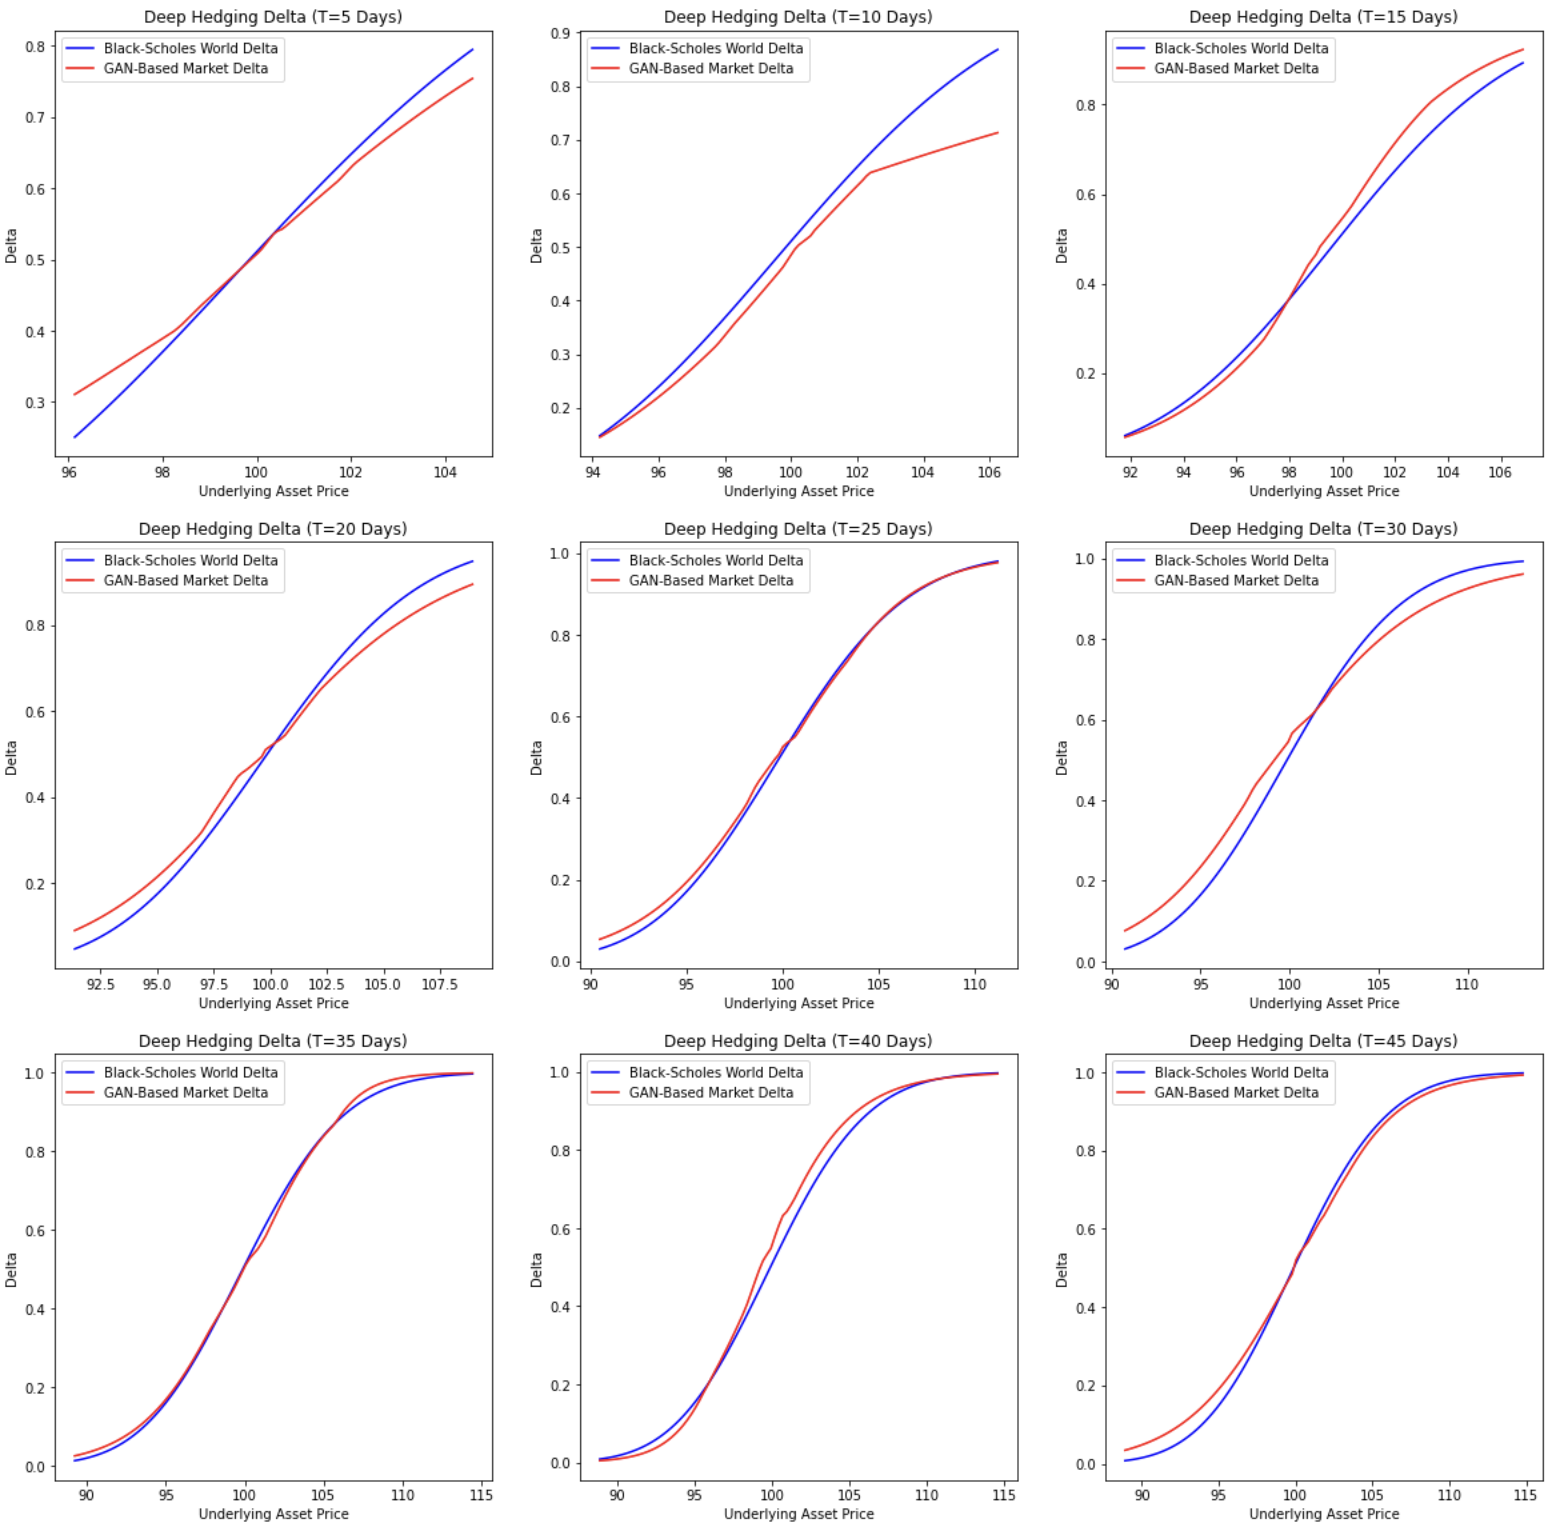
\includegraphics[width=14cm]{templates/assets/drl/delta.png}
\caption{Deltas for Deep Hedging Over Time (Black-Scholes vs. GAN)}
\end{figure}

\noindent As shown in the distribution of PnLs in Figure 3-6, it appears that deep hedging has more consistent returns using AI-generated data than Black-Scholes simulations, as the returns are more thinly spread when trained on a GAN-based market. Furthermore, it can be seen in Figure 3-7 that using GAN-based market simulation results in a smaller overall delta for various underlying prices. This implies that the deep hedging algorithm was able to reduce the delta risk exposure and sensitivity to underlying price movements of the portfolio using AI-generated market data instead of a parametric Black-Scholes simulation. 
\\\\
To have a robust hedging strategy, the PnLs of the portfolio should have consistently low volatility in different market scenarios. The volatilities of the returns for the strategy should be relatively stable across different market simulations so that the deep hedging agent can perform consistently and handle various market risks in the real world. The distribution and kernel density estimate (KDE) for the volatility of hedged returns for deep hedging on a Black-Scholes world and GAN-based market environment for an option with strike $K=100$ are displayed below.
\begin{figure}[h]
\centering
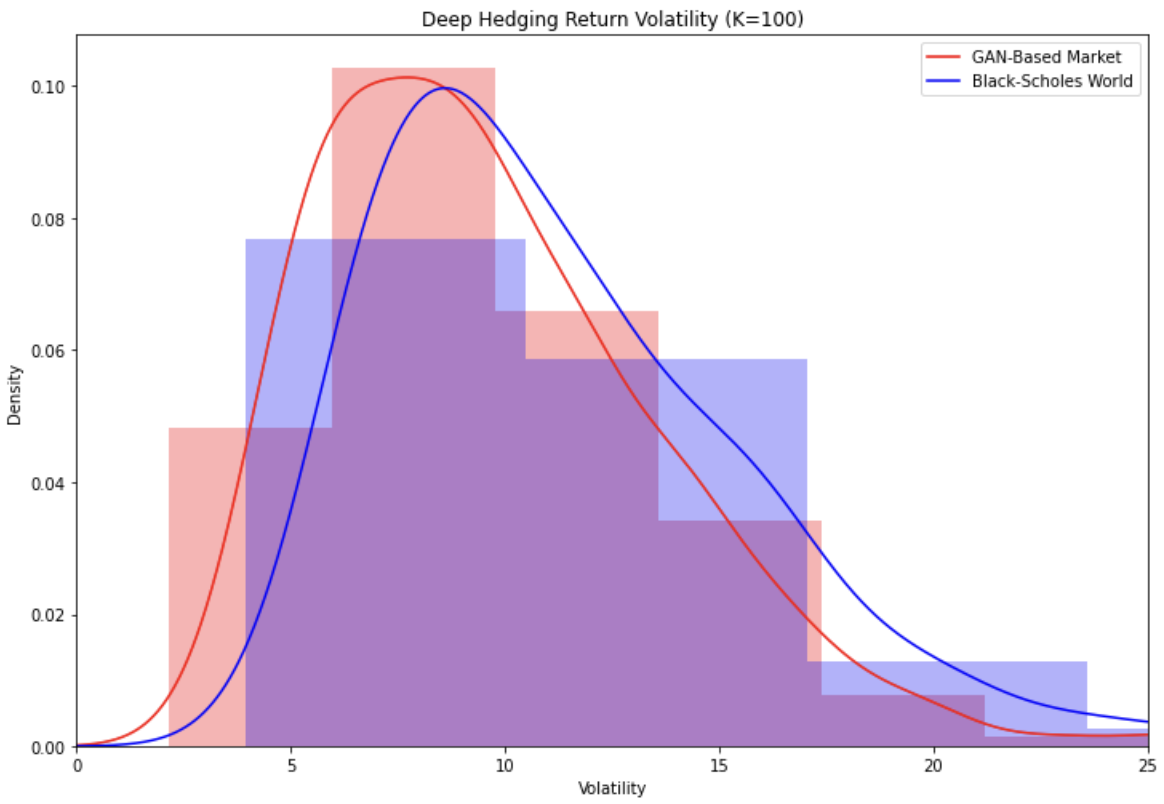
\includegraphics[width=13.5cm]{templates/assets/drl/hedge_return_volatility.png}
\caption{Histogram of Deep Hedged Return Volatility (Black-Scholes vs. GAN)}
\end{figure}

\begin{table}[h]
\begin{centering}
\begin{tabular}{@{\extracolsep{2pt}}lcccccc}
\toprule
Return Volatility & Mean   & Median \\ \midrule
Black-Scholes Market &   11.72          &   5.75    \\
GAN-Based Market  &     9.72        &    4.26  \\
\bottomrule
\end{tabular}
\caption{Distribution of Deep Hedged Return Volatility (Black-Scholes vs. GAN)}
\end{centering}
\end{table}

\noindent Observing the results of using a Black-Scholes and a GAN-based market environment for training deep hedging methods, it appears the latter produces a more robust hedging policy for reducing volatility against various market risks and conditions. Across all the simulations, the hedging strategy PnLs and volatilities are more thinly spread in the GAN-based market. The GAN is likely capturing specific properties of financial data that cannot be modeled by parametric methods like Monte Carlo simulations. Overall, it appears that the AI-generated data allows deep hedging agents to better learn the market structure and make more consistent hedging decisions. Overall, these results are promising for traders and investors to use deep hedging in the real world to manage real market risks.
\\ \\
This demonstrates the practicality of using AI-generated data in training and developing machine learning methods for derivatives pricing and dynamic hedging, and potentially for other financial applications as well. Although there is still more work to be done in optimizing the GAN in learning the underlying market data distribution and experimenting with different deep reinforcement learning algorithms, this proof-of-concept framework removes the need for market assumptions by learning directly from data. Since this system is model-free and data-driven, there is great potential for using GANs and deep reinforcement learning to hedge risks in other asset classes as well. The multi-agent deep reinforcement learning and GAN-based market simulation system provides a flexible and scalable framework for investors to systematically hedge a portfolio of diverse assets in a complex market with various risks, frictions, and constraints using historical data.